\chapter{Конструкторская часть}

\section{Требования к программному обеспечению}

Программа должна предоставить следующие функции:
\begin{itemize}
    \item создание сцены заданного размера;
    \item добавление, поворот, удаления объектов сцены;
    \item перемещение, поворот камеры сцены.
\end{itemize}

\section{Алгоритм, использующий z-буфер}

\begin{itemize}
    \item Всем элементам буфера кадра присвоить фоновое значение.
    \item Инициализировать z-буфер минимальным значением глубины.
    \item Для каждого полигона сцены в произвольном порядке:	
    \begin{itemize}
        \item для каждого пикселя, который принадлежит полигону вычислить глубину z(x, y); 
        \item cравнить вычисленную глубину пикселя со значением, которое хранится в z-буфере. 
        Если Z(x, y) > Zbuf (x, y), то Zbuf (x, y) = Z(x, y) и color(x, y) = pixelColor. 
    \end{itemize}
    \item Вывести итоговое изображение.
\end{itemize}

На рисунке \ref{img:zbuf} представлена схема алгоритма для удаления 
невидимых линий и поверхностей с помощью z-буфера. 

\clearpage
\begin{figure}[h]
    \centering
    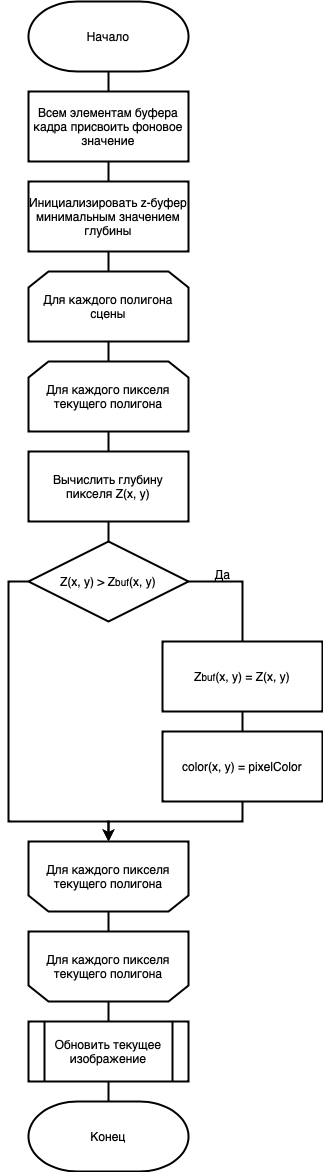
\includegraphics[width=0.4\linewidth]{img/zbuf.png}
    \caption{Схема алгоритма, использующего z-буфер}
    \label{img:zbuf}
\end{figure}
\noindent

\clearpage

\section{Алгоритм для построения теней, использующий z-буфер}

\begin{itemize}
    \item Для каждого направленного источника света:
    \begin{itemize}
        \item инициализировать теневой z-буфер минимальным значением глубины; 
        \item определить теневой z-буфер для источника. 
    \end{itemize}
    \item Выполнить алгоритм z-буфера для точки наблюдения. 
    При этом, если некоторая поверхность оказалась видимой относительно 
    текущей точки наблюдения, то проверить, видима ли данная точка со стороны 
    источников света. 
    \item Для каждого источника света: 
    \begin{itemize}
        \item координаты рассматриваемой точки (x, y, z) преобразовать 
        из вида наблюдателя в координаты (x0, y0, z0) в вид из рассматриваемого источника света; 
        \item cравнить значение ZshadowBuf(x0,y0) со значением Z0(x0,y0). 
        Eсли Z0(x0, y0) < ZshadowBuf (x0, y0), то пиксел высвечивается с учетом его затемнения, 
        иначе точка высвечивается без изменений. 
    \end{itemize}
    \item Вывести итоговое изображение.
\end{itemize}

На рисунках~\ref{img:shadow1} -- \ref{img:shadow2} представлена схема алгоритма для построения теней с помощью z-буфера.

\begin{figure}[h]
    \centering
    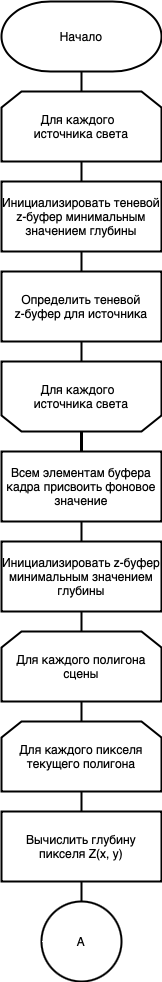
\includegraphics[width=0.23\linewidth]{img/shadow1.png}
    \caption{Схема алгоритма для построения теней, использующего z-буфер}
    \label{img:shadow1}
\end{figure}
\noindent

\begin{figure}[h]
    \centering
    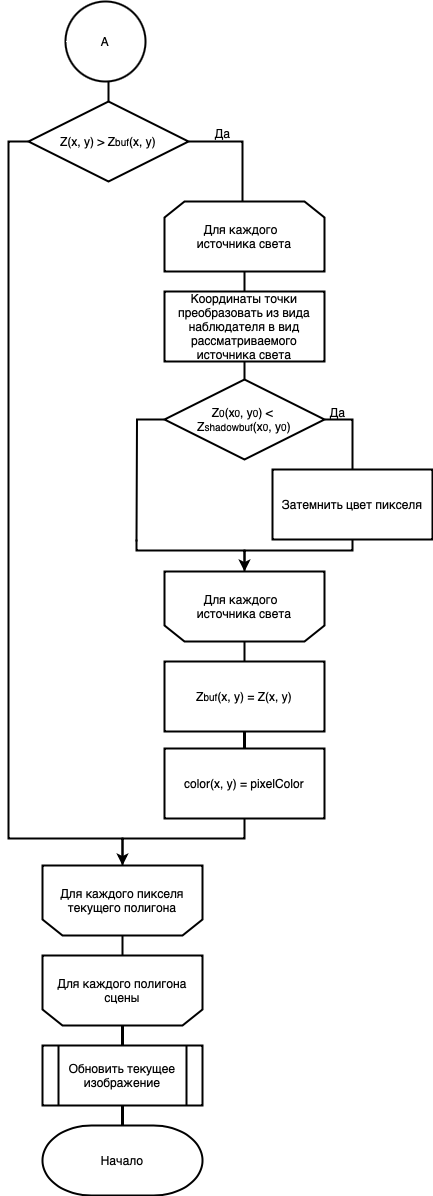
\includegraphics[width=0.5\linewidth]{img/shadow2.png}
    \caption{Схема алгоритма для построения теней, использующего z-буфер}
    \label{img:shadow2}
\end{figure}
\noindent

\clearpage
\section{Используемые типы и структуры данных для представления объектов}

Для решения поставленных задач курсового проекта необходимо опре- делить представление объектов разрабатываемой программы. 
В таблице \ref{tab:object} представлены объекты и выбранные для них типы и структуры данных.

\begin{table}[!ht]
    \centering
    \caption{\label{tab:object}Выбранный типы и структуры данных для представления объектов}
    \begin{tabular}{|p{6cm}|p{10cm}|}
    \hline
        Объект & Типы и структуры данных \\ \hline
        Точка в трехмерном пространстве & Вектор, состоящий из четырех координат типа float64: x, y, z, w  \\ \hline
        Вершина & Точка в трехмерном пространстве \\ \hline
        Полигон & Структура, содержащая три вершины \\ \hline

        Камера &  Структура, содержащая направление и матрицу преобразования вершины
        в пространство камеры вершины в пространство камеры типа float64 \\ \hline

        Двигатель программы &  Структура, содержащая: камеру,
        источник света, z-буфер, теневой буфер, 
        матрицу типа float64 для преобразования из пространства
        камеры в пространство источника света\\ \hline
    \end{tabular}
\end{table}

\section*{Вывод}
В этом разделе были определены требования к программному обеспечению, выбраны типы и структуры данных. Также были разработаны 
алгоритм для удаления невидимых линий и поверхностей, использующий z-буфер и алгоритм, для построения теней с помощью z-буфера.
